\documentclass[12pt,oneside]{article}

\usepackage{graphicx}
\usepackage[pagebackref,linktocpage,breaklinks,colorlinks,%
linkcolor=black,anchorcolor=black,citecolor=black,%
filecolor=black,menucolor=black,runcolor=black,%
urlcolor=black]{hyperref}

\usepackage[spanish]{babel}
\usepackage[utf8]{inputenc}

\newcommand{\doublequote}[1]{``#1''}

\begin{document}
	\begin{center}
		\huge\bf
		Respuestas a las Preguntas de Discusión de la Tesis
	\end{center}

	\vspace{0.4in}
	\noindent\textbf{\Large Título del trabajo de diploma:}\\
	\large Generación Automática de Ontologías\\\\
	\textbf{\Large Nombre y apellidos del estudiante:}\\
	\large José Ariel Romero Costa\\\\
	\textbf{\Large Nombre y apellidos del tutor:}\\
	\large MSc. Juan Pablo Consuegra Ayala

	\vspace{0.2in}
	\section{Respuestas al tribunal}
	\begin{enumerate}
		\item Diga de entre todas las partes de la metodología propuesta, cuál considera que es la componente más débil, que más influye negativamente en la calidad de los resultados, y por qué.

		\item[R)] Considero que la componente más débil y que más influye negativamente en la calidad de los resultados es el concepto con rol \doublequote{\textit{Reference}}. Esto se debe a que los conceptos de este tipo no tienen significado semántico específico y su función es hacer referencia a otro concepto. Esto lo convierte en un concepto sin valor para la base de conocimiento, y por tanto, de las relaciones donde estas participan no puede extraerse conocimiento relevante.

		\item A partir de la respuesta a la pregunta anterior, proponga una estrategia concreta para mejorar dicha componente.

		\item[R)] Esta componente puede mejorar dándole solución al problema de las correferencias. Al resolver esto, los nodos de tipo \doublequote{\textit{Reference}} desaparecen de la ontología, y las relaciones de estos pasan a ser relaciones de la correferencia de cada uno de ellos. Esto reduce la cantidad de nodos en el grafo, dado que las correferencias de cada uno de ellos es un concepto, entonces existe al menos un nodo en la base de conocimiento para cada nodo del tipo \doublequote{\textit{Reference}} que representa semánticamente la correferencia de este. A la vez, aumenta la cantidad de conocimiento representado en el grafo y la calidad de esto, debido a que la cantidad de relaciones que había anteriormente se conservan, ya que solo pasaron a pertenecer a otro nodo. Además, estas relaciones pueden interactuar con las restantes de cada nodo asociado, lo que potencialmente aumentaría la cantidad de conocimiento representado como se mencionó anteriormente.
	\end{enumerate}

	\section{Respuestas al oponente}
	\begin{enumerate}
		\item Realice una comparación entre su metodología para construir el grafo de conocimiento y los principales sistemas de \textit{ontology learning} existentes.

		\item[R)] Durante la última década, varias técnicas de los campos de procesamiento de lenguaje natural, aprendizaje automático, recuperación de información, procesamiento de datos y representación del conocimiento contribuyeron al avance del desarrollo de ontologías.

		En la figura \ref{figure:ontology_learning_methodology}\cite{ref:1} se aprecia, paso a paso, el proceso de aprendizaje de ontologías y algunas técnicas que pueden usarse en cada uno de esos pasos.

		\begin{figure}[h!]
			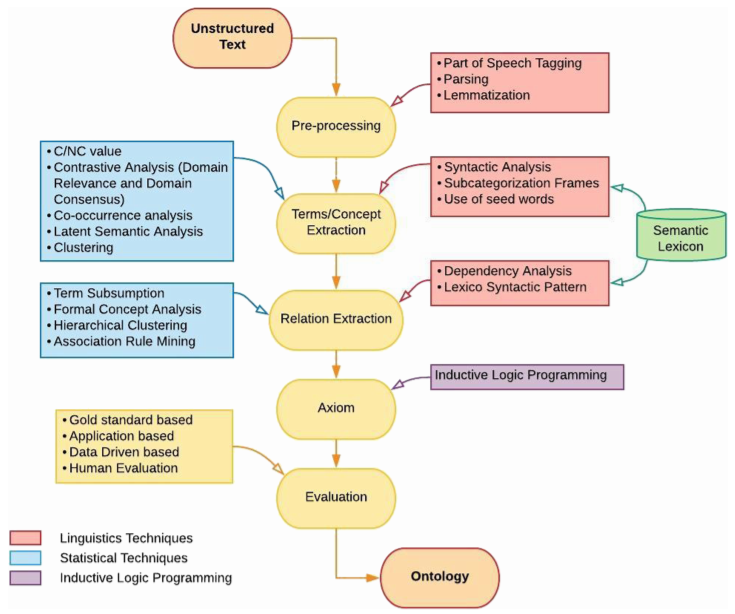
\includegraphics[width=\linewidth]{graphics/ontology_learning_methodology.png}
			\caption{Metodología de aprendizaje de ontologías}
			\label{figure:ontology_learning_methodology}
		\end{figure}

		El proceso llevado a cabo en la investigación realizada abarca los dos últimos pasos: \textit{axiomas} y \textit{evaluación}. Mientras el o los corpus anotados usados como base no fue objeto de estudio, y estos abarcan los tres primeros pasos: \textit{preprocesamiento}, \textit{extracción de términos/conceptos} y \textit{extracción de relaciones}.

		Además, en el proceso de creación de la base de conocimiento, se lleva a cabo la normalización de términos, pero no se resuelven las correferencias. Esto último también es usual realizarlo, y es un proceso que normalmente es llevado a cabo con aprendizaje automático. Prescindir de este proceso posibilitó la creación de un algoritmo con el uso de ordenamiento topológico, dando ventaja en cuanto a la complejidad temporal y espacial respecto al de aprendizaje automático.

		La evaluación de la ontología se realizó basada en datos, aunque para ello se utilizó un único corpus para ambos procesos: la creación y la verificación de la ontología. Para llevar a cabo esto de forma satisfactoria, se dividieron las oraciones de este corpus en dos conjuntos disjuntos, uno de entrenamiento, con el cual se crea la base de conocimientos y otro de verificación, para realizar la evaluación con este.

		Resultado final de la comparación: siendo honestos y autocríticos, ya sea por un motivo o por otro, los cuales no son objetivo de debate en este documento, el proceso llevado a cabo crea una ontología a partir de un corpus de documentos anotados. Pero no resuelve las correferencias, lo cual hace que la ontología creada no tenga representado todo el conocimiento existente en estos documentos. Además, para ser un \doublequote{verdadero} o \doublequote{clásico} proceso de \textit{ontology learning}, como el mostrado en la figura \ref{figure:ontology_learning_methodology}, se necesita trabajar en otros enfoques e implementar otros algoritmos y/o ideas para enriquecer la investigación. Esto la convierte en un estudio incompleto y que deja las puertas abiertas para el trabajo futuro en este.

		\item Realice una evaluación cualitativa, por expertos, de la ontología obtenida a partir de todo el corpus, y evalúe la calidad del conocimiento generado.

		\item[R)] Debido al poco tiempo con el que se cuenta para llevar a cabo este proceso, y dado que la base de conocimiento resultante de esta investigación contiene $4,935$ nodos y $8,623$ relaciones entre ellos, no es posible llevar a cabo este proceso. No se pudo gestionar con un grupo de expertos la revisión de esta base de conocimiento porque esta tiene dominio médico, y en este tiempo de coronavirus los médicos son la principal línea de defensa y están sumamente ocupados. Por otra parte, parte del conocimiento representado es de conocimiento general, con lo cual hubiera podido haber hecho yo la evaluación manual, pero como se mencionó anteriormente, la gran cantidad de nodos y relaciones imposibilitó esto. En cambio, se dará una metodología genérica que puede ser usada para llevar a cabo una evaluación por expertos.

		Primeramente, se recomienda la participación de un grupo de expertos en el mismo dominio al de la base de conocimiento. Mientras más grande sea este grupo, más rápido pudiera llevarse a cabo esta evaluación. Una forma para la distribución de los conceptos y relaciones a revisar puede ser ordenar alfabéticamente los conceptos, y si se cuenta con $N$ expertos entonces dividir el grupo de conceptos en $N$ fragmentos continuos, de esta forma se garantiza un intervalo de revisión \doublequote{fácil} de recordar y de saber qué se ha revisado ya y qué queda por revisar; siempre y cuando cada uno de estos grupos se revisado por orden alfabético también. De cada grupo, se revisa el concepto en sí y las relaciones que parten de este, pero no las que llegan a él. De esta forma, se garantiza la revisión de todos los conceptos, puesto que inicialmente todos los conceptos fueron ordenados y distribuidos, y se garantiza también la revisión de todas las relaciones, dado que toda relación tiene su origen en algún concepto, y este concepto será revisado por algún experto, por tanto, la relación será revisada.

		La evaluación por expertos es considerada la más completa y de la cual se pueden evaluar y extraer una mayor cantidad de criterios, estadísticas, entre otros~\cite{ref:1}. Criterios específicos de evaluación pueden verse en Brewster \textit{et al.} \cite{ref:7}, donde se propone \textit{densidad} e \textit{intermediación}. Además, Guarino y Welty \cite{ref:8} evalúan las ontologías a través de un sistema conocido como \doublequote{\textit{OntoClean}}. Este sistema está basado en un conjunto de criterios que comprenden identidad, esencia y unidad. Ellos usan estos criterios para caracterizar y explorar el significado sugerido por clases, relaciones y propiedades que realmente tienen relevancia al construir una ontología específica.

		\item Proponga una estrategia para resolver el problema de correferencias.

		\item[R)] Para resolver las correferencias puede hacerse un clasificador que dado dos conceptos o menciones $m_i$ y $m_j$ en el documento, determine si son correferentes o no. Para llevar a cabo este proceso, es necesario un corpus de entrenamiento, donde esté bien definido qué conceptos son referencias y a quién hace referencia.

		\newpage

		Para este proceso puede ser extraído varios \textit{features} de cada pareja de conceptos, como por ejemplo:

		\begin{itemize}
			\item[•] Coincidencia exacta:\\
			son $m_i$ y $m_j$ la misma cadena exacta luego de eliminar sus superficialidades?, las superficialidades pueden ser, por ejemplo, articulos, conjugaciones, número\dots

			\item[•] Gramática:\\
			$g\acute{e}nero_i$, $g\acute{e}nero_j$, $n\acute{u}mero_i$, $n\acute{u}mero_j$, $pronombre_i?$, $pronombre_j?$

			\item[•] Semántica:\\
			clase semántica del concepto

			\item[•] Posicional:\\
			distancia entre ambos conceptos; por ejemplo, medida en cantidad de palabras
		\end{itemize}

		Luego de entrenar el modelo, puede ser usado, clasificando así cada pareja de conceptos o menciones, en si son correferentes o no. Pero este enfoque puede tener un problema, que no cumpla con la transitividad. Es decir, si $A$ es correferente de $B$ y $B$ es correferente de $C$ puede que no detecte que $A$ es correferente de $C$. Para resolver este último problema, es valido procesar las parejas de conceptos de izquierda a derecha, y cada vez que se identifique una pareja $m_i$, $m_j$, se establece un enlace o \textit{link} entre el concepto y su referente. De esta forma se crea un árbol de correferencias, donde la raíz es el concepto principal y los demás son correferencias a este.

		Otras vías de resolución de este problema puede ser por medio de \cite{ref:4}, \cite{ref:5} y \cite{ref:3}. Para llevar a cabo estas ideas, puede ser necesario reentranar el o los modelos ofrecidos en el idioma español. Para hacer esto, pudiera necesitarse un corpus de entrenamiento~\cite{ref:6} y algunos otros recursos presentes en la web, como por ejemplo, el uso de \textit{word embeddings}.

		\item Dado que en una ontología el contenido aparece usualmente sintetizado o resumido, ¿puede proponer una estrategia, aplicable a su metodología, para resumir contenido?

		\item[R)] Para resumir el contenido en la ontología, puede llevarse a cabo de forma simultánea a la creación de esta, un proceso similar al ofrecido en \doublequote{\textit{Gathering object interactions as semantic knowledge}}\cite{ref:2} basado en el mismo corpus de documentos. Al realizar esto, se puede asumir la palabra representativa de cada \textit{cluster} como igual a las palabras contenidas en este. Por tanto, todas las relaciones en la ontología entre palabras pertenecientes a un \textit{cluster}, serán \doublequote{movidas} a las relaciones de la palabra representativa del \textit{cluster}. Además, se añade una relación \textit{same-as} entre cada palabra en el \textit{cluster} y su elemento representativo en el mismo. Con esto, se sintetiza el conocimiento de todas las relaciones en la ontología entre palabras de un mismo \textit{cluster} en el conocimiento expresado por la palabra representativa de este. Este proceso puede reducir potencialmente la cantidad de nodos y aristas existentes en el grafo de conocimiento, mientras que el conocimiento en sí, queda resumido.
	\end{enumerate}

	\newpage

	\bibliographystyle{acm}
	\bibliography{bibliography}
\end{document}